\documentclass[a4paper,12pt,twoside]{book}
\usepackage[utf8]{inputenc}
\usepackage{amssymb}
\usepackage{amsmath}
\usepackage{graphicx}
\usepackage{siunitx}
\usepackage{gensymb}
\usepackage[numbers,compress]{natbib}
\usepackage{chapterbib} % For chapter-specific bibliographies
\usepackage{subcaption}
\usepackage{times} % Times font, consider using newtxtext if needed
\usepackage{geometry}
\usepackage{setspace}
\usepackage{tocloft}
\usepackage{ragged2e}
\usepackage{array}
\usepackage{fancyhdr}
\usepackage{titlesec}
\usepackage{hyperref} % Load hyperref last
\usepackage{url}
\usepackage{pgfplots}
\usepackage{tabularx}
\usepackage{multirow}
\usepackage{tabularray}
\usepackage{longtable}
\usepackage{helvet}

\usepackage[T1]{fontenc}
\usepackage{tikz}
%\usepackage{lipsum}
\usepackage{afterpage}
\usepackage{pdflscape}
\usepackage{adjustbox}
\usepackage{multicol}
\usepackage{mathtools}
\usepackage{chemformula}
\usepackage{bm}
\usepackage{lscape}
\usepackage[version=4]{mhchem}

\renewcommand{\thefootnote}{\fnsymbol{footnote}}

\newgeometry{top=1in, outer=1in, bottom=1in, inner=1.5in}

\graphicspath{{figures/}} % Set the path for figures

% Define the chapter format to keep title and text on the same page
\titleformat{\chapter}[display]
  {\normalfont\fontsize{22}{22}\bfseries\centering} % Title font and centering
  {\chaptertitlename\ \thechapter}{0pt}{} % Chapter number and title format [] % No space after title (you can add some space here if needed, like [\vspace{10pt}]) 

% Modify spacing for chapter, section, subsection, etc.
\titlespacing*{\chapter}{0pt}{0pt}{20pt} %{<command>}{<left>}{<before-sep>}{<after-sep>}
\titlespacing*{\section}{0pt}{8pt}{5pt}
\titlespacing*{\subsection}{0pt}{8pt}{5pt}
\titlespacing*{\subsubsection}{0pt}{8pt}{5pt}

% Modify TOC formatting
\renewcommand{\cftchapleader}{\cftdotfill{\cftdotsep}}
\renewcommand\contentsname{\centerline{TABLE OF CONTENTS}}

% Fancyhdr setup
\pagestyle{fancy}
\cfoot{\thepage}
\rhead{}
\lhead{}
\renewcommand{\headrulewidth}{0pt}
\renewcommand{\footrulewidth}{0pt}

\hyphenpenalty=10000
\exhyphenpenalty=10000

\begin{document}
\sloppy
\frontmatter
\addtocontents{toc}{\textbf{Title}\hfill\textbf{Page No.}\par}
\begin{titlepage}

\begin{center}
{\sffamily

\fontsize{20pt}{24pt}\selectfont \textbf{Long Title of Thesis}\\
\vspace{12pt}
\fontsize{16pt}{20pt}\selectfont by
\\
\vspace{12pt}
\textbf{XXXXXXXXXX\\Registration No.: YYYYYYYYYYY}
\\
\vspace{24pt}
A thesis submitted to the\\
Academy of Scientific \& Innovative Research\\
for the award of the degree of\\
DOCTOR OF PHILOSOPHY
\\
in
\\
SCIENCE
\\
\vspace{24pt}
Under the supervision of
\\
\textbf{Dr. XXXXXXXXX}
\\
%\bigskip

\includegraphics[width=1.25in]{CSIR-Logo.png}
\\
\textbf{Name of Institute}
\\
%\bigskip

\includegraphics[width=1.75in]{AcSIR-Logo.jpg}
\\
Academy of Scientific and Innovative Research
\\
AcSIR Headquarters, CSIR-HRDC campus\\
Sector 19, Kamla Nehru Nagar\\
Ghaziabad, U.P. – 201 002, India
\\
\vspace{24pt}
\textbf{2025}

}
\end{center}

\end{titlepage}
\newpage
\thispagestyle{empty}
\mbox{}
\newpage
\addtocounter{page}{-2}
\thispagestyle{plain}
\begin{center}
\fontsize{16pt}{24pt}\selectfont \textbf{Certificate}
\end{center}
\hline

\vspace{0.3cm}
\fontsize{12pt}{24pt}\selectfont

This is to certify that the work incorporated in this Ph.D. thesis entitled, \textbf{“Long title of Thesis”}, submitted by \textbf{XXXXXXXXX} to the Academy of Scientific and Innovative Research (AcSIR) in fulfillment of the requirements for the award of the Degree of \textbf{Doctor of Philosophy}, embodies original research work carried-out by the student. We, further certify that this work has not been submitted to any other University or Institution in part or in full for the award of any degree or diploma. Research materials obtained from other sources and used in this research work have been duly acknowledged in the thesis. Images, illustrations, figures, tables, etc., used in the thesis from other sources, have also been duly cited and acknowledged.

\vspace{3cm}
\begin{table}[h]
\centering
\fontsize{12pt}{18pt}\selectfont
\begin{tabular}{p{8.5cm}p{4.5cm}}
(Signature of Student) & (Signature of Supervisor)\\
Name: \textbf{XXXXXXXX} & Name: \textbf{Dr. XXXXXXXXX}\\
 
Date:  & Date: \\
\end{tabular}
\end{table}


%\newpage
\newpage
\thispagestyle{empty}
\mbox{}
\newpage
\thispagestyle{plain}
\begin{center}
\fontsize{16pt}{24pt}\selectfont \textbf{Statements of Academic Integrity}
\end{center}
\hline

\vspace{0.3cm}
\fontsize{12pt}{24pt}\selectfont I \textbf{XXXXXXXX}, a Ph.D. student of the Academy of Scientific and Innovative Research (AcSIR) with Registration No. \textbf{YYYYYYYY} hereby undertake that, the thesis entitled \textbf{“Long Title of Thesis”} has been prepared by me and that the document reports original work carried out by me and is free of any plagiarism in compliance with the UGC Regulations on \emph{“Promotion of Academic Integrity and Prevention of Plagiarism in Higher Educational Institutions (2018)”} and the CSIR Guidelines for \emph{“Ethics in Research and in Governance (2020)”}.

\vspace{3cm}
\begin{table}[h]
\centering
\fontsize{12pt}{18pt}\selectfont
\begin{tabular}{p{9cm}p{5cm}}
 & \textbf{Signature of the student}\\
 & Date: \\
 & Place: \\
\end{tabular}
\end{table}
\hline
\vspace{0.3cm}
\fontsize{12pt}{24pt}\selectfont It is hereby certified that the work done by the student, under my supervision, is plagiarism-free in accordance with the UGC Regulations on \emph{“Promotion of Academic Integrity and Prevention of Plagiarism in Higher Educational Institutions (2018)”} and the CSIR Guidelines for \emph{“Ethics in Research and in Governance (2020)”}.

\vspace{3cm}
\begin{table}[h]
\centering
\fontsize{12pt}{18pt}\selectfont
\begin{tabular}{p{9cm}p{5cm}}
 & \textbf{Signature of the Supervisor}\\
 & Name: \\
 & Date: \\
 & Place: \\
\end{tabular}
\end{table}

%\newpage
\newpage
\thispagestyle{empty}
\mbox{}
\newpage
\thispagestyle{empty}
\vspace*{\fill}

\begin{center}
\fontsize{16pt}{24pt}\selectfont \textbf{Dedication}
\end{center}
\fontsize{12pt}{24pt}\selectfont \emph{To those who inspired this journey and will never read this.}
\vspace*{\fill}

\newpage
\thispagestyle{empty}
\vspace*{\fill}
\begin{center}
\fontsize{12pt}{24pt}\selectfont \emph{"When life gives you lemons, construct a crude electrochemical battery" - Unknown}
\end{center}
\vspace*{\fill}
\newpage
\addcontentsline{toc}{chapter}{Acknowledgement}
\thispagestyle{plain}
\begin{center}
\textbf{\textbf{\fontsize{16pt}{24pt}\selectfont Acknowledgement}}
\end{center}

\vspace{0.3cm}
\fontsize{12pt}{18pt}\selectfont 

Acknowledgement here

\begin{flushright}
\textbf{Your Name}
\end{flushright}

\newpage
\addcontentsline{toc}{chapter}{Samgraham}
\thispagestyle{plain}

\begin{flushleft}
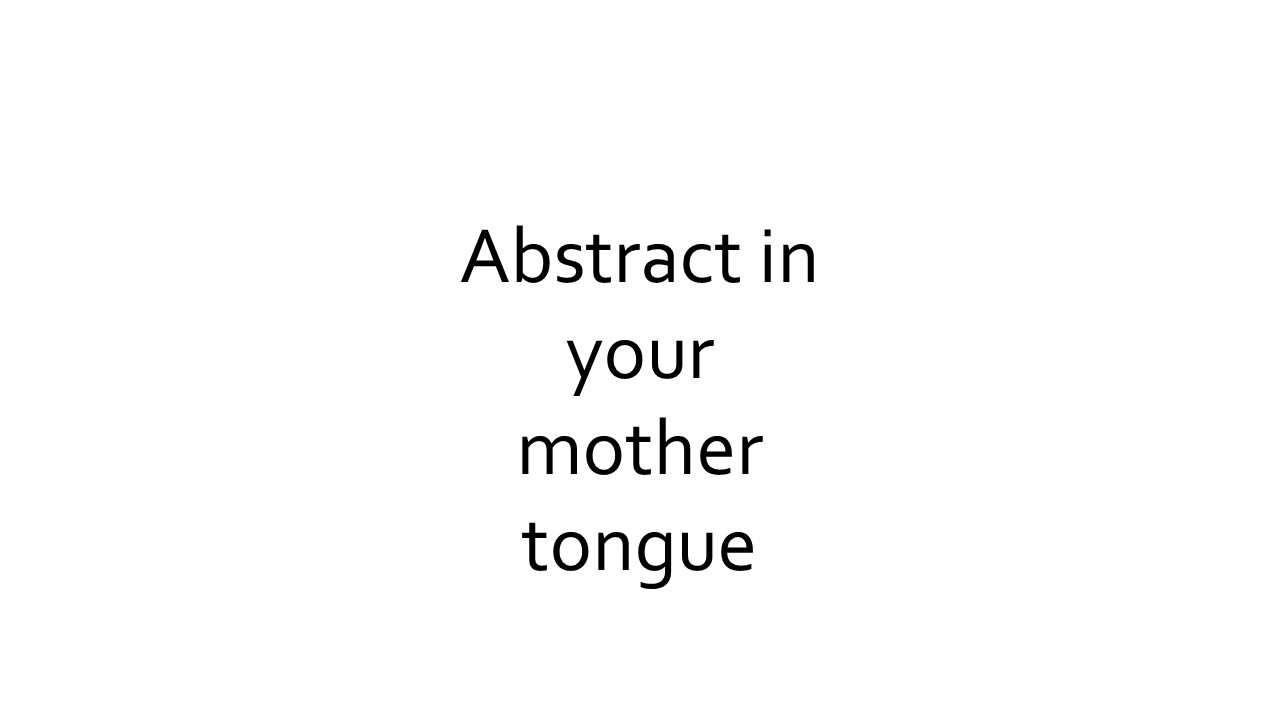
\includegraphics[width=6in]{samgraham.jpg}
\end{flushleft}

\newpage


\newpage
\addcontentsline{toc}{chapter}{Table of Contents}
\tableofcontents
\newpage
\addcontentsline{toc}{chapter}{List of Tables}
\listoftables
\newpage
\addcontentsline{toc}{chapter}{List of Figures}
\listoffigures
\newpage
\addcontentsline{toc}{chapter}{List of Abbreviations}
\thispagestyle{plain}
\begin{flushleft}
\textbf{\textbf{\fontsize{22pt}{22pt}\selectfont Abbreviations}}
\end{flushleft}

%\vspace{0.3cm}
% Please add the following required packages to your document preamble:
% \usepackage{longtable}
% Note: It may be necessary to compile the document several times to get a multi-page table to line up properly
\begin{longtable}{ll}
\normalsize
\label{tab:abbreviations}\\
AC & Alternating Current \\
AFM & Atomic Force Microscopy \\
DC & Direct Current \\
FESEM & Field Emission Scanning Electron Microscope \\
GITT & Galvanistatic Intermittent Titration Technique \\
HSE & Hybrid Solid Electrolyte \\
IL & Ionic Liquid \\
LAGP & Lithium Aluminium Germanium Phosphate, Li$_{1+x}$Al$_{x}$Ge$_{2-x}$(PO$_{4}$)$_{3}$ \\
MS & Mass Spectroscopy \\
NASICON & Sodium (Na) Super Ion Conductor \\
OCP & Open Circuit Potential \\
PAN & Polyacrylonitrile \\
QSE & Quasi-Solid Electrolyte \\
RTIL & Room Temperature Ionic Liquid \\
SCE & Solid Composite Electrolyte \\
TPU & Thermoplastic Polyurethane \\
UTM & Universal Testing Machine \\
XRD & X-Ray Diffraction
\end{longtable}

\newpage
 
\mainmatter
\onehalfspacing % Set line spacing to 1.5
\graphicspath{ {figures/introduction/} }
\chapter{Introduction}

Write main matter of chapter here \cite{kurian2024pursuit}

%\section{Introduction}
%\section{Experimental section}
%\section{Results and discussion}
%\section{Inferences}
\begin{figure}[!ht]
\centering

\includegraphics[width=\textwidth]{introduction.jpg}
\caption{}
\label{fig:introduction}
\end{figure}


\renewcommand{\bibsection}{\section*{References}}
\bibliography{introductionrefs.bib}
\bibliographystyle{unsrt} %completed
\graphicspath{ {figures/methodology/} }
\chapter{Methodology}

Write main matter of chapter here \cite{kurian2024pursuit}

%\section{Introduction}
%\section{Experimental section}
%\section{Results and discussion}
%\section{Inferences}
\begin{figure}[!ht]
\centering

\includegraphics[width=\textwidth]{methodology.jpg}
\caption{}
\label{fig:methodology}
\end{figure}


\renewcommand{\bibsection}{\section*{References}}
\bibliographystyle{unsrt}
\bibliography{methodologyrefs.bib}

  %completed
\graphicspath{ {figures/chapter1/} }
\chapter{Short Title of Chapter 1}
\begin{center}
\fontsize{18pt}{0.6cm}\selectfont \textbf{Long Title of Chapter 1\footnote[2]{This work has been peer reviewed and published: \textit{\textbf{Ionics}}, 2022, 28(\textbf{6}):2649-2660}}
\end{center}

\section*{\large Abstract}
Write abstract here

\newpage

Write main matter of chapter here \cite{sampathkumar2022influence}
%\section{Introduction}
%\section{Experimental section}
%\section{Results and discussion}
%\section{Inferences}
\begin{figure}[!ht]
\centering

\includegraphics[width=\textwidth]{chapter1.jpg}
\caption{}
\label{fig:chapter1}
\end{figure}


\renewcommand{\bibsection}{\section*{References}}
\bibliography{chapter1refs.bib}
\bibliographystyle{unsrt}  %completed
\graphicspath{ {figures/chapter2/} }
\chapter{Short Title of Chapter 2}
\begin{center}
\fontsize{18pt}{0.6cm}\selectfont \textbf{Long Title of Chapter 2\footnote[2]{This work has been peer reviewed and published: \textit{\textbf{Journal of Energy Storage}}, 2025, \textbf{115}:115882}}
\end{center}

\section*{\large Abstract}
Write abstract here

\newpage

Write main matter of chapter here \cite{kurian2025thermoplastic}

%\section{Introduction}
%\section{Experimental section}
%\section{Results and discussion}
%\section{Inferences}
\begin{figure}[!ht]
\centering

\includegraphics[width=\textwidth]{chapter2.jpg}
\caption{}
\label{fig:chapter2}
\end{figure}


\renewcommand{\bibsection}{\section*{References}}
\bibliography{chapter2refs.bib}
\bibliographystyle{unsrt}  %completed
\graphicspath{ {figures/chapter3/} }
\chapter{Short Title of Chapter 3}
\begin{center}
\fontsize{18pt}{0.6cm}\selectfont \textbf{Long Title of Chapter 3\footnote[2]{This work has been peer reviewed and published: \textit{\textbf{Physica B: Condensed Matter}}, 2021, \textbf{615}:413087}}
\end{center}

\section*{\large Abstract}
Write abstract here

\newpage

Write main matter of chapter here \cite{shafi2021effect}

%\section{Introduction}
%\section{Experimental section}
%\section{Results and discussion}
%\section{Inferences}

\begin{figure}[!ht]
\centering

\includegraphics[width=\textwidth]{chapter3.jpg}
\caption{}
\label{fig:chapter3}
\end{figure}


\renewcommand{\bibsection}{\section*{References}}
\bibliography{chapter3refs.bib}
\bibliographystyle{unsrt}  %completed
\graphicspath{ {figures/} }
\chapter{Conclusion}

Main matter of conclusion here 
%\section{Summary}
%\subsubsection*{Key highlights:}
\begin{figure}[!ht]
\centering

\includegraphics[width=\textwidth]{conclusion.jpg}
\caption{}
\label{fig:conclusion}
\end{figure}

  %not started
\newpage
\addcontentsline{toc}{chapter}{Abstract}
\thispagestyle{plain}
\begin{center}
\textbf{\textbf{\fontsize{16pt}{24pt}\selectfont Abstract}}
\end{center}
\vspace{0.3cm}
\hline

\fontsize{12pt}{12pt}\selectfont 
\begin{longtable}{@{}p{0.45\linewidth} p{0.55\linewidth}@{}}
Name of the Student: \textbf{XXXX XXXXXX} & Registration No.: \textbf{YYYYYYYYYYYY} \\
Faculty of Study: \textbf{Physical Science} & Year of Submission: \textbf{2025} \\
AcSIR academic center / CSIR Lab: \textbf{ZZZZZZZZZZ} & Name of the Supervisor: \textbf{Dr. XXXXXX} \\
\multicolumn{2}{@{}p{\linewidth}@{}}{Title of the thesis: \textbf{Long Title of Thesis}} \\
\end{longtable}
\hline
\vspace{1cm}

\fontsize{12pt}{12pt}\selectfont 
Thesis abstract here
\addcontentsline{toc}{chapter}{Appendix-I: List of Publications in SCI Journals emanating from the thesis work}
\chapter*{Appendix I}

\subsection*{List of Publications in SCI Journals emanating from the thesis work}
\vspace{1cm}
\begin{enumerate}
\item \textbf{Evan Kurian}, Jayashree Pitchai, Soundarya Neelanarayanan, Deepak Kumar, Sellamuthu N. Jaisankar, and K. Ramesha. ”Thermoplastic polyurethane (TPU) based high-performing solid polymer electrolytes for solid-state lithium metal batteries.” \textit{Journal of Energy Storage} 115 (2025): 115882

\item \textbf{Evan Kurian}, Jayashree Pitchai, Soundarya Neelanarayanan, and K. Ramesha. ”In Pursuits of All Solid State Batteries (ASSB): Advances at the Cathode-Electrolyte Interface for Garnet-Based ASSB.” \textit{RSC Applied Interfaces} 1.5 (2024): 868-89

\item Sampathkumar, Ramakumar, M. G. Babu, \textbf{Evan Kurian}, R. N. Ramesha, Dasari Bosubabu, and K. Ramesha. ”Influence of lithium metal anode coated with a composite quasi-solid electrolyte on stabilizing the interface of all-solid-state battery.” \textit{Ionics} (2022): 1-12.

\item \textbf{Evan Kurian}, Jayashree Pitchai, Deepak Kumar, Shreya Jose, and K. Ramesha. ”Plasticizer-Assisted Garnet LLZO Integration in TPU-based Solid Composite Electrolytes for High-Performance Solid-State Lithium Metal Batteries.” \textit{Manuscript accepted}
\end{enumerate}

 %completed
\addcontentsline{toc}{chapter}{Appendix-II: List of Papers presented in National / International conferences}
\chapter*{Appendix II}

\subsection*{List of Papers presented in National / International conferences}
\vspace{1cm}
\subsubsection{1. Presented paper}
\textbf{Title:} Thermoplastic Polyurethane (TPU) based high-performing Solid Polymer Electrolytes for Solid-State Lithium Metal Batteries \\
\textbf{Conference:} 13th International Symposium on Advances in Electrochemical Science and Technology (iSAEST-13), January 8-10, 2025, Thiruvananthapuram, Kerala, India\\
\textbf{Abstract:}\\
Abstract here

\vspace{1cm}
\subsubsection{2. Presented poster}
\textbf{Title:} Influence of lithium metal anode coated with a composite quasi-solid electrolyte on stabilizing the interface of all-solid-state battery \\
\textbf{Conference:} International Conference on Energy Conversion and Storage (IECS-2023), 18-20 January 2023, Research Park, IIT Madras, Chennai, India\\
\textbf{Abstract:}\\
Abstract here %completed
\end{document}
